%%
%% Copyright 2007-2020 Elsevier Ltd
%% 
%% This file is part of the 'Elsarticle Bundle'.
%% ---------------------------------------------
%% 
%% It may be distributed under the conditions of the LaTeX Project Public
%% License, either version 1.2 of this license or (at your option) any
%% later version.  The latest version of this license is in
%%    http://www.latex-project.org/lppl.txt
%% and version 1.2 or later is part of all distributions of LaTeX
%% version 1999/12/01 or later.
%% 
%% The list of all files belonging to the 'Elsarticle Bundle' is
%% given in the file `manifest.txt'.
%% 

%% Template article for Elsevier's document class `elsarticle'
%% with numbered style bibliographic references
%% SP 2008/03/01
%%
%%
%% $Id: elsarticle-template-num.tex 190 2020-11-23 11:12:32Z rishi $
%%
%%
\documentclass[preprint,12pt]{elsarticle}

%% Use the option review to obtain double line spacing
%% \documentclass[authoryear,preprint,review,12pt]{elsarticle}

%% Use the options 1p,twocolumn; 3p; 3p,twocolumn; 5p; or 5p,twocolumn
%% for a journal layout:
%% \documentclass[final,1p,times]{elsarticle}
%% \documentclass[final,1p,times,twocolumn]{elsarticle}
%% \documentclass[final,3p,times]{elsarticle}
%% \documentclass[final,3p,times,twocolumn]{elsarticle}
%% \documentclass[final,5p,times]{elsarticle}
%% \documentclass[final,5p,times,twocolumn]{elsarticle}

%% For including figures, graphicx.sty has been loaded in
%% elsarticle.cls. If you prefer to use the old commands
%% please give \usepackage{epsfig}

%% The amssymb package provides various useful mathematical symbols
\usepackage{amssymb}
\usepackage{amsmath}
\usepackage[pdftex]{hyperref}
%% The amsthm package provides extended theorem environments
%% \usepackage{amsthm}

%% The lineno packages adds line numbers. Start line numbering with
%% \begin{linenumbers}, end it with \end{linenumbers}. Or switch it on
%% for the whole article with \linenumbers.
%% \usepackage{lineno}

\journal{LCCV}

\begin{document}
	
	\begin{frontmatter}
		
		%% Title, authors and addresses
		
		%% use the tnoteref command within \title for footnotes;
		%% use the tnotetext command for theassociated footnote;
		%% use the fnref command within \author or \address for footnotes;
		%% use the fntext command for theassociated footnote;
		%% use the corref command within \author for corresponding author footnotes;
		%% use the cortext command for theassociated footnote;
		%% use the ead command for the email address,
		%% and the form \ead[url] for the home page:
		%% \title{Title\tnoteref{label1}}
		%% \tnotetext[label1]{}
		%% \author{Name\corref{cor1}\fnref{label2}}
		%% \ead{email address}
		%% \ead[url]{home page}
		%% \fntext[label2]{}
		%% \cortext[cor1]{}
		%% \affiliation{organization={},
			%%             addressline={},
			%%             city={},
			%%             postcode={},
			%%             state={},
			%%             country={}}
		%% \fntext[label3]{}
		
		\title{Axial vibration of a continuum bar using MPM}
		
		%% use optional labels to link authors explicitly to addresses:
		%% \author[label1,label2]{}
		%% \affiliation[label1]{organization={},
			%%             addressline={},
			%%             city={},
			%%             postcode={},
			%%             state={},
			%%             country={}}
		%%
		%% \affiliation[label2]{organization={},
			%%             addressline={},
			%%             city={},
			%%             postcode={},
			%%             state={},
			%%             country={}}
		
		\author[inst1]{Lorran Ferreira Oliveira}
		
		\affiliation[inst1]{organization={Universidade Federal de Alagoas},%Department and Organization
			addressline={Av. Lourival Melo Mota, Tabuleiro do Martins}, 
			city={Maceió},
			postcode={57072-970}, 
			state={AL},
			country={Brazil}}
		
		\begin{abstract}
			%% Text of abstract
			The Material Point Method (MPM) is a numerical simulation technique that describes the approximate behavior of continuum materials. The MPM discretizes the body domain $\Omega$ into a finite set of $n_p$ particles and places them in a mesh that spans the entire solution domain. Velocities, masses and forces are mapped to mesh nodes, where they are updated with an explicit temporal integration process. These quantities are mapped back to the particles and the mesh configuration is then restored to its initial state. For educational purpose, this work describes objectively the process of solving a free vibration problem of a continuum uniaxial bar by MPM. The discretized solution was implemented using Python and the results were validated with the analytical solution.
		\end{abstract}
		
		\begin{keyword}
			%% keywords here, in the form: keyword \sep keyword
			Material Point Method \sep Computational Mechanics \sep Dynamics \sep Free Vibration
			%% PACS codes here, in the form: \PACS code \sep code
		\end{keyword}
		
	\end{frontmatter}
	
	%% \linenumbers
	
	%% main text
	\section{Introduction}
	A continuous body in motion has state variables that vary over time, and the Finite Element Method (FEM) is one of the most commonly used numerical tools in industry and academia with the purpose of describing these variations. However, the FEM, which tracks changes in state variables with a Lagrangian approach, has important limitations when dealing with problems involving large deformations \cite{zhang_material_2017}. Using FEA, these analyzes can suffer from a problem called mesh entanglement. This problem occurs when there is a large distortion in the mesh that discretizes the domain, which implies an increase in the error in the interpolations made by the shape functions that approximate the continuum solution \cite{SINAIE2017}.

    The MPM emerged as one of the alternatives to the FEM for the treatment of problems with large deformations. The method consists of discretizing the solution domain into a set of particles that individually carry their own state variables (mass, velocity, density and volume, for example). The state variables quantities are mapped from the particles to the background mesh nodes and then updated to a time step $\Delta t$. The updated information is then returned to the particles and the background mesh is restored to its initial state \cite{zhang_material_2017}.
        
    

	%% The Appendices part is started with the command \appendix;
	%% appendix sections are then done as normal sections
	\section{The Material Point Method}
	
    In continuum mechanics, the conservation of momentum of a body is described in its strong and weak forms by the expressions (\ref{eq:eq_momentum_strong}) and (\ref{eq:eq_momentum_weak}), respectively.

	\begin{equation}
		\rho\, \dot{\boldsymbol{u}}-\nabla\boldsymbol{\sigma}-\rho\, \boldsymbol{b}=0
		\label{eq:eq_momentum_strong}
	\end{equation}

	\begin{equation}
		\int_{\Omega} \rho\, \ddot{\boldsymbol{u}}\, \delta\dot{\boldsymbol{u}}\, d\boldsymbol{x}-\int_{\Omega}\nabla\boldsymbol{\Bar{\sigma}}\, \delta\dot{\boldsymbol{u}}\, d \boldsymbol{x} - \int_{\Omega} \rho\, \boldsymbol{b}\, \delta\dot{\boldsymbol{u}}\, d \boldsymbol{x}=0
		\label{eq:eq_momentum_weak}
	\end{equation}
	
	\noindent Where $\boldsymbol{\sigma}$ is the stress tensor, $\boldsymbol{\Bar{\sigma}}$ is the specific stress tensor  $\boldsymbol{\Bar{\sigma}}=\frac{\boldsymbol{\sigma}}{\rho}$, $\boldsymbol{b}$ is the body forces vector and $\delta \dot{\boldsymbol{u}}$ is the variation of velocity.
	
    Up to this point, there is no distinction between MPM and MEF \cite{bathe_finite_2014}. However, from the process of discretization of the problem (\ref{eq:eq_momentum_weak}) these differences become evident \cite{zhang_material_2017}. In MPM the density $\rho$ is approximated by
	
	\begin{equation}
	    \rho(\boldsymbol{x},t)=\sum_p m_p\,\delta(\boldsymbol{x} - \boldsymbol{x}^t_p)
	\end{equation}
	
    \noindent Where $\delta$ is the Dirac Delta, $m_p$ is the mass of the particle $p$ and $\boldsymbol{x}_p^t$ is the position of the particle $p$ at the instant $t$ .

    The procedure for updating the state variables of the particles for each time step can be done by calculating the stresses before (Update Stress First - USF) or after the temporal integration process in the nodes of the background mesh (Update Stress Last - USL) \cite{zhang_material_2017}. The USL, unlike the USF, is a naturally dissipative solution, which gives more stability to the numerical process \cite{bardenhagen_energy_2002}.
	
    Adopting the USL update scheme, the mass $m_p$, the momentum and the internal forces are mapped from particles to nodes of the background mesh according to the expressions (\ref{eq:part_to_node_mass}), (\ref{eq:part_to_node_momentum}) and (\ref{eq:part_to_node_force}).
	
	\begin{equation}
		m_{n}^{t} = \sum_{p}m_{p}^{t}\, N_{np}(\boldsymbol{x}_{p}^{t})
		\label{eq:part_to_node_mass}
	\end{equation}
	
	\begin{equation}
		\textbf{p}_{n}^{t} = \sum_{p}m_{p}^{t}\, \dot{\textbf{u}}_{p}^{t}\, N_{np}(\boldsymbol{x}_{p}^{t})
		\label{eq:part_to_node_momentum}
	\end{equation}
	
	\begin{equation}
		\textbf{f}_{n}^{\,t} = -\sum_{p}V_{p}^{t}\, \boldsymbol{\Bar{\sigma}}_{p}^{t}\, \nabla N_{np}(\textbf{x}_{p}^{t})
		\label{eq:part_to_node_force}
	\end{equation}
	
	\noindent Where $N_{np}(\boldsymbol{x}_p^t)$ is the shape function (\ref{eq:shape}) evaluated in the position of the particle $\boldsymbol{x}_p^t$ in the instant $t$.
	
	\begin{equation}
	    N_{np}(\boldsymbol{x}_p^t) = \left\{\begin{matrix}
                        1-\frac{|\boldsymbol{x}_p^t-\boldsymbol{x}_n|}{L} \qquad \text{if}\,\, |\boldsymbol{x}_p^t-\boldsymbol{x}_n|\leq L\\
                        0 \qquad\qquad \text{otherwise} 
                 \end{matrix}\right.
        \label{eq:shape}
	\end{equation}  
	
	\begin{equation}
	    \nabla N_{np}(\boldsymbol{x}_p^t) = \left\{\begin{matrix}
                        1 \qquad \qquad \qquad \text{if}\,\, (\boldsymbol{x}_n - L) \leq \boldsymbol{x}_p^t \leq \boldsymbol{x}_n \\
                        -1 \qquad \qquad \qquad \text{if}\,\, (\boldsymbol{x}_n + L) \geq \boldsymbol{x}_p^t > \boldsymbol{x}_n \\
                        0 \qquad\qquad \text{otherwise} 
                 \end{matrix}\right.
        \label{eq:shape_diff}
	\end{equation}  
	
    Then, the nodal moments are updated by the expression (\ref{eq:update_momentum}).
    
	\begin{equation}
		\boldsymbol{p}_{n}^{t+\Delta t} = \boldsymbol{p}_{n}^{t}+\boldsymbol{f}_{n}^{\,t}\, \Delta t
		\label{eq:update_momentum}
	\end{equation}
	
	The imposition of displacement constraints on fixed nodes is done by canceling the moments and forces acting on these nodes (equations (\ref{eq:p_fix}) and (\ref{eq:f_fix})).
	
	\begin{equation}
		\boldsymbol{p}_{n_{fix}}^{t+\Delta t}=0
		\label{eq:p_fix}
	\end{equation}
	
	\begin{equation}
		\boldsymbol{f}_{n_{fix}}^{\,t+\Delta t}=0
	    \label{eq:f_fix}
	\end{equation}
	
	At this point, the background mesh nodes have all the information about the state variables updated for the instant $t+\Delta t$. These quantities are therefore mapped back to the particles by the equations (\ref{eq:vp}) and (\ref{eq:xp}). 
	
	\begin{equation}
		\boldsymbol{v}_{p}^{t+\Delta t}=\boldsymbol{v}_{p}^{t} +\Delta t \sum_{n}\frac{N_{np}(\boldsymbol{x}_{p}^{t})\boldsymbol{f}_{n}^{\,t}}{m_{n}^{t}}
		\label{eq:vp}
	\end{equation}

	\begin{equation}
		\boldsymbol{x}_{p}^{t+\Delta t}=\boldsymbol{x}_{p}^{t}+\Delta t \sum_{n} \frac{N_{np}(\boldsymbol{x}_{p}^{t})\,\boldsymbol{p}_{n}^{t+\Delta t}}{m_{n}^{t}}
	    \label{eq:xp}
	\end{equation}

    After updating the velocities and positions of the particles, the volume (\ref{eq:V}) and the internal stresses of these particles (\ref{eq:sigma}) are updated as a function of the deformation gradient (\ref{eq:F}) and the velocity gradient (\ref{eq:L}), respectively.

	\begin{equation}
		\textbf{L}_{p}^{t+\Delta t}=\sum_{n} \nabla N_{np}(\boldsymbol{x}_{p}^{t})\,\boldsymbol{v}_{n}^{t+\Delta t}
		\label{eq:L}
	\end{equation}

	\begin{equation}
		\textbf{F}_{p}^{t+\Delta t}=(\textbf{I}+\textbf{L}_{p}^{t+\Delta t}\,\Delta t)\textbf{F}_{p}^{t}
        \label{eq:F}
	\end{equation}
	
	\begin{equation}
	    V_p^{t+\Delta t}=det(\textbf{F}_p^{t+\Delta t})\,V_p^0
	    \label{eq:V}
	\end{equation}
	
	\begin{equation}
	    \boldsymbol{\sigma}_p^{t+\Delta t}=\boldsymbol{\sigma}_p^t + \Delta \boldsymbol{\sigma}_p
        \label{eq:sigma}
	\end{equation}
	
	\noindent Where $\textbf{I}$ is the identity matrix, $\textbf{L}_p^{t+\Delta t}$ is the velocity gradient, $\textbf{F}_p^{t+\Delta t}$ is the deformation gradient, $V_p^0$ is the initial volume of the particle $p$ and $V_p^{t+\Delta t}$ is the particle volume in the instant $t+\Delta t$.
	
	After the update of the stress tensor, the background mesh is restored to its initial configuration.

	\section{Results}
	    Consider the problem proposed by \cite{bardenhagen_energy_2002} which consists of a continuum uniaxial bar of length $L$, fixed at $x=0$ and free at $x=L$, elastic modulus $E$ and density $\rho $. Adopting as initial condition velocities that excite the vibration mode $m$, calculated by (\ref{eq:v_ini}), the velocity of this bar at its center of mass is given by the expression (\ref{eqs:vcm}).
	    
	    \begin{equation}
	        v(x,0)=v_0\,\sin(\beta_m\,x)
	        \label{eq:v_ini}
	    \end{equation}
	    
	    \begin{equation}
		    v_{cm}(t)=\frac{v_{0}}{\beta_{m}\,L}\cos(\omega_{m}\,t)
		    \label{eqs:vcm}
	    \end{equation}
	    
	    \noindent Where $\beta_m$ and $\omega_m$ depend on the excited vibration mode $m$ and are calculated, respectively, by (\ref{eq:beta_m}) and (\ref{eq:omega_m}).
	    
	    \begin{equation}
		    \beta_{m}=\frac{\pi(2m-1)}{2L}	
		    \label{eq:beta_m}
	    \end{equation}
	    
        \begin{equation}
            \omega_m=\beta_m\,c
            \label{eq:omega_m}
        \end{equation}
        
        \noindent Where 
        
        \begin{equation}
            c = \sqrt{\frac{E}{\rho}}
            \label{eq:c}
        \end{equation}


	The Python 3.11.0 programming language was used to develop the solution, available in this \textit{\href{https://github.com/lorranfoliveira/mini_mpm}{github repository}}, to the presented problem. The numerical simulation by MPM was performed with data adopted by \cite{bardenhagen_energy_2002}: $E=100$, $\rho=1$, $L=25$, $v_0=0.1$ and $\Delta t=0.1\frac{L}{c}$. The bar domain was divided into $25$ elements of length $L_e=1$ and $50$ particles were used for discretization of the body (two particles per element). Figure (\ref{fig:domain}) illustrates the initial configuration of the discretized structure.
	
	\begin{figure}
    	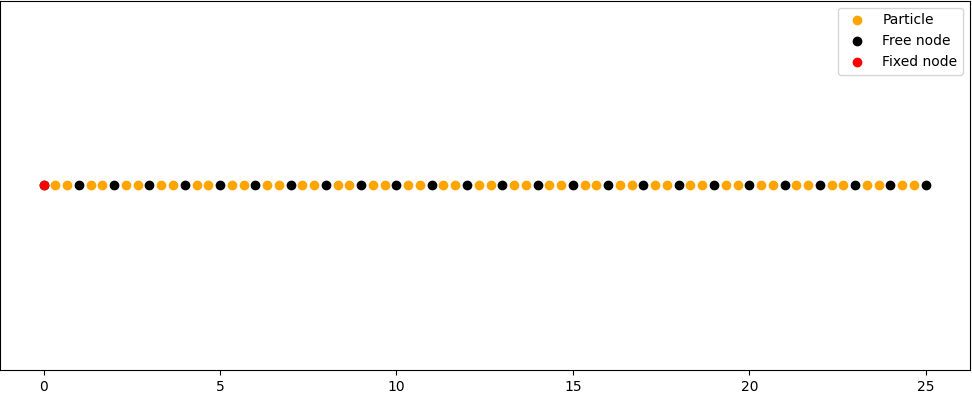
\includegraphics[width=\linewidth]{exemplo_dominio.png}
    	\caption{Initial structure discretization. The structure is discretized into 50 uniformly distributed particles (2 particles per element). All particles are free to move only in the direction of the principal axis. Yellow dots represent particles, black dots represent free nodes, and red dots represent fixed nodes.}
    	\centering
    	\label{fig:domain}
    \end{figure}
    
    \begin{figure}
    	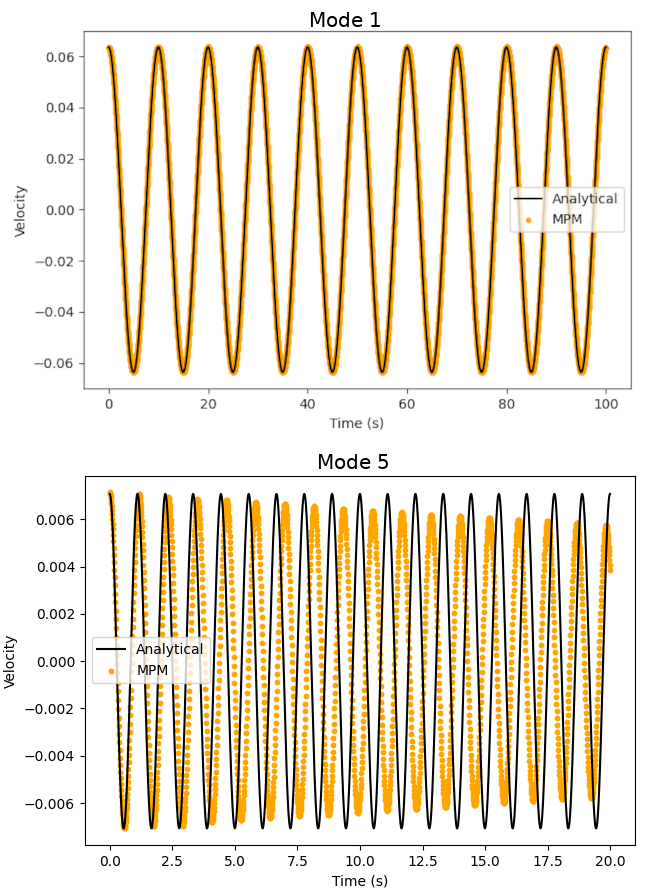
\includegraphics[width=10cm]{results.png}
    	\centering
    	\caption{Vibration mode 1: The continuum black line represents the analytical solution obtained by the expression (\ref{eqs:vcm}) and describes the velocity of the bar's center of mass as a function of time. The yellow dots represent the discrete solutions obtained by the implemented MPM.}
    	\label{fig:results}
    \end{figure}
    
    \begin{figure}
    	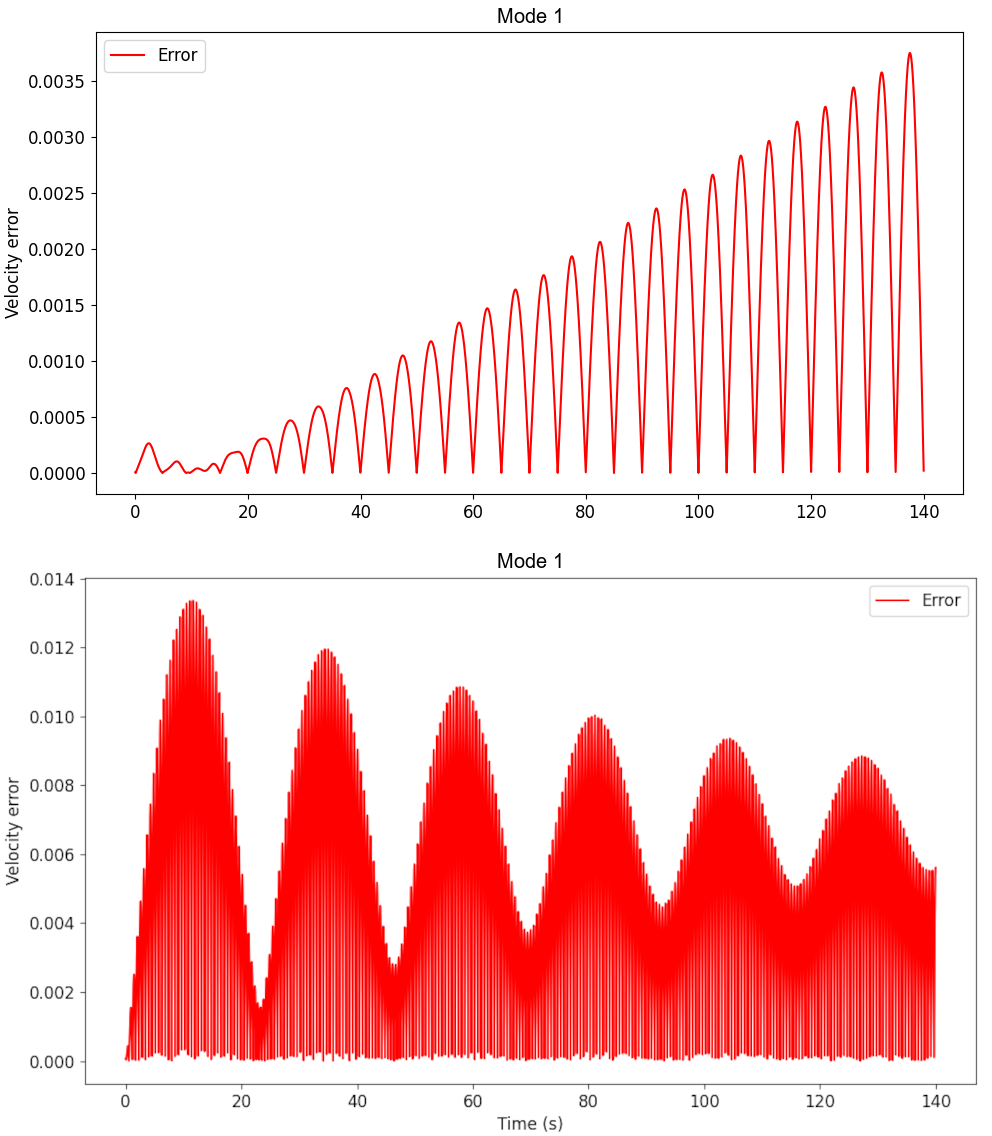
\includegraphics[width=10cm]{error.png}
    	\centering
    	\caption{Numerical error: The error was calculated as the modulus of the difference between the numerical and analytical solutions. Because of the use of the USL as a solution strategy, the system naturally dissipates energy, as can be seen in the two graphs.}
    	\label{fig:error}
    \end{figure}
    
    The Figure (\ref{fig:results}) shows the evolution bar velocity in its center of mass over time for the vibration modes $m=1$ and $m=5$. The results obtained by the implementation made are compatible whith the analytical solution (\ref{eqs:vcm}). For $m=5$, note that there is a dissipation in the energy that makes the analytical solution different from the numerical one. However, this damped vibration is expected and it is caused by the use of USL. These results, including the dumped one, are compatible with the literature \cite{bardenhagen_energy_2002}.
    
    Figure (\ref{fig:error}) shows the error of the numerical solution implemented in relation to the analytical expression (\ref{eqs:vcm}). Note that the energy dissipation resulting from the application of the USL is perceived by the increase in the error with time, both for mode 1 and for mode 5. However, in mode 5 a larger periodic oscillation in the error is noticeable, and this occurs due to to the fact that the numerical solution goes out of phase for this case, therefore increasing the error for short periods of time. However, in general, there is an increase in error as a function of time for the two analyzed vibration modes.
	
	\section{Conclusion}
	An introductory study to MPM was carried out with the development of an educational code to solve the problem of free vibration of a uniaxial bar. The solution found by MPM, implemented with the USL update strategy, proved to be compatible with the known analytical solution when $m=1$. For $m=5$, a damping effect appears in the system, in addition to an out-of-phase vibration. However, such behaviors are expected and compatible with numerical solutions
    found in the literature.


	%% If you have bibdatabase file and want bibtex to generate the
	%% bibitems, please use
	%%
	
	\bibliographystyle{elsarticle-num} 
	\bibliography{refs}
	
	%% else use the following coding to input the bibitems directly in the
	%% TeX file.
	
	%%\begin{thebibliography}{00}
		

		
		% \bibitem{}
		
	%%\end{thebibliography}
\end{document}
\endinput
%%
%% End of file `elsarticle-template-num.tex'.
